\documentclass[11pt,a4paper]{article}

\usepackage[margin=1in]{geometry}
\usepackage[T1]{fontenc}
\usepackage[utf8]{inputenc}
\usepackage{lmodern}
\usepackage{hyperref}
\usepackage{array}
\usepackage{graphicx}
\usepackage{float}
\graphicspath{{report/figures/}{figures/}}

\hypersetup{
    colorlinks=true,
    linkcolor=black,
    citecolor=black,
    urlcolor=blue
}

\linespread{1.06}
\emergencystretch=2em

\title{\vspace{-1.2em}Progress Report and Request for Suggestions\\
\large Weather-Aware Travel Itinerary Optimization as a Publishable Research Project}
\author{Prepared for Prof. Liyan Xie\\[0.5em] [Your Name]}
\date{June 2026}

\begin{document}

\maketitle

\section*{Message to Prof. Xie}

\noindent Dear Prof. Xie,

\vspace{0.5em}

\noindent I hope you are doing well. I am writing to share the current progress of my weather-aware travel itinerary optimization project and to ask whether you might be willing to give me suggestions on how to strengthen it as a publishable research project. CHI 2027 is one possible target if the work is framed around human-centered decision support, but I am also open to other venues that may fit the final contribution better.

The project started from my IE 5533 final report, where I built a data-driven itinerary optimization pipeline for urban travel planning. Since then, I have extended it substantially. The current system is no longer only a Santa Barbara route optimizer. It now supports configurable multi-day trip scenarios, hotel/base-city decisions, nature-aware preference controls, statewide California route experiments, a hybrid bandit plus Gurobi repair method, validation scripts, and a multi-page interactive dashboard with customer, research, and evaluation views.

The current repository is available as a \href{https://github.com/Ztang-Yit-Xiaang/weather-aware-travel-itinerary-optimization}{GitHub project}.

At the same time, the project has several unresolved problems. Some are technical, such as data sparsity, fallback-source provenance, and how to interpret solver fallback states in the evaluation dashboard. Others are research-oriented, such as how to evaluate user trust, agency, and explanation quality in an itinerary-planning system. I would be very grateful for your advice on how to narrow the research contribution, improve the methodology, decide which problems are most important, and identify suitable paper submission venues.

\vspace{0.5em}

\noindent Sincerely,\\
\mbox{[Your Name]}

\newpage

\section*{1. Project Goal}

\noindent The central goal is to build a travel-planning system that does more than rank attractions. Instead, the system should generate feasible multi-day itineraries under real constraints:

\begin{itemize}
    \item limited daily time and total trip budget;
    \item travel time between attractions, hotels, and base cities;
    \item weather exposure and expected waiting time;
    \item traveler pace, such as relaxed, balanced, or explorer;
    \item personal interest tradeoffs among nature, city, culture, and history;
    \item hotel/base-city selection and possible overnight relocation;
    \item route diversity so the plan does not become repetitive.
\end{itemize}

\noindent My longer-term research direction is to turn this into a nationwide planning framework. In that version, lightweight agents would help at the beginning of the workflow by finding, fetching, and organizing destination-specific datasets. However, the route itself would still be generated by explicit optimization methods, not by free-form language-model generation. The intended architecture is therefore agent-assisted data preparation plus optimization-controlled route generation.

\section*{2. What the IE 5533 Final Report Already Established}

\noindent The final report established the first working version of the system. Its main procedure was:

\begin{enumerate}
    \item Collect candidate attractions from Yelp-style business data, using ratings, review counts, categories, and geographic coordinates.
    \item Construct a baseline attraction utility score from rating and review volume.
    \item Retrieve historical weather features from Open-Meteo, including temperature, precipitation, rain flags, cold flags, weekends, and seasonal variables.
    \item Use review-density patterns as a proxy for attraction demand and waiting time.
    \item Train a predictive model, mainly XGBoost, to estimate weather-aware congestion or waiting-time effects.
    \item Estimate visit duration and cost using attraction-category heuristics.
    \item Construct travel-time matrices among attractions, and later among hotels and attractions.
    \item Formulate the trip as a multi-day Tourist Trip Design Problem with mixed-integer decision variables.
    \item Solve route choices using CP-SAT and Gurobi-style optimization formulations.
    \item Export static and interactive maps for route interpretation.
\end{enumerate}

\noindent The main conceptual contribution of that version was the shift from recommendation as ranking to recommendation as constrained route planning.

\section*{3. Progress Since the Final Report}

\subsection*{3.1 Configurable Planning Pipeline}

\noindent The project has been reorganized into a reusable Python package. The current workflow is driven by configuration files such as the default trip config and the nature trip config. This allows trip length, budget, scenario, traveler profile, interest profile, and nature settings to be changed without rewriting the notebook.

\subsection*{3.2 Expanded Scenario Support}

\noindent The original workflow focused mainly on a California coastal/Santa Barbara case. The current system supports multiple scenarios:

\begin{itemize}
    \item California coast;
    \item California statewide nature;
    \item Las Vegas plus national parks;
    \item New York City plus nature.
\end{itemize}

\noindent For the California statewide nature scenario, the system now represents large outdoor regions such as Yosemite, Sequoia, Kings Canyon, Joshua Tree, Death Valley, Lake Tahoe, Point Reyes, Pinnacles, Lassen Volcanic, Redwood National and State Parks, and Big Sur. These are modeled as nature regions with gateway/base cities, rather than only as isolated POIs.

\subsection*{3.3 Separation of Pace and Interest}

\noindent A major improvement is that traveler pace is separated from traveler interest. Pace is represented by profiles such as relaxed, balanced, and explorer. Interest is represented by a continuous bar:

\[
p = [p_{\mathrm{nature}}, p_{\mathrm{city}}, p_{\mathrm{culture}}, p_{\mathrm{history}}],
\qquad p_k \geq 0,\quad \sum_k p_k = 1.
\]

\noindent This makes the model more expressive. For example, a relaxed traveler can still prefer national parks, and an explorer can still prefer museums and city attractions.

\subsection*{3.4 Nature-Aware Utility}

\noindent The system now adds interest-adjusted utility. In simplified form:

\[
\begin{array}{rl}
u_i^{\mathrm{interest}} = &
u_i^{\mathrm{base}}
+ \lambda_{\mathrm{fit}} p^\top a_i
+ \lambda_{\mathrm{park}} \mathrm{parkBonus}_i \\[0.25em]
& - \lambda_{\mathrm{weather}} \mathrm{weatherRisk}_i
- \lambda_{\mathrm{season}} \mathrm{seasonRisk}_i
- \lambda_{\mathrm{detour}} \mathrm{detourMinutes}_i .
\end{array}
\]

\noindent This allows national parks, scenic viewpoints, protected areas, detour burden, and weather sensitivity to affect route selection.

\subsection*{3.5 Hierarchical and Hybrid Optimization}

\noindent The current system uses several planning methods:

\begin{itemize}
    \item ranking and greedy baselines;
    \item MCDA and TOPSIS-style scoring;
    \item Bayesian/UCB candidate selection;
    \item epsilon-constrained Gurobi routing;
    \item hierarchical Gurobi planning;
    \item hybrid bandit selection plus small Gurobi route repair.
\end{itemize}

\noindent The hybrid method is important because a nationwide route problem will be too large for one monolithic solver. The current direction is to use candidate selection and hierarchical decomposition first, then apply exact or near-exact optimization on smaller route subproblems.

\subsection*{3.6 Interactive Map and Dashboard Outputs}

\noindent The system exports:

\begin{itemize}
    \item lightweight share maps;
    \item full interactive dashboards with customer and research/test modes;
    \item a separate evaluation dashboard for method-comparison charts and solver tradeoff notes;
    \item selected route GeoJSON;
    \item POI JSON;
    \item hotel-choice artifacts;
    \item nature exploration layers;
    \item validation and artifact-size reports.
\end{itemize}

\noindent The dashboard also has a browser-side preview mechanism. Users can adjust interest weights and see approximate score changes quickly. Customer controls load saved route artifacts or clearly labeled browser previews. The full optimized route, however, still requires rerunning the Python optimization pipeline.

\subsection*{3.7 Tool-First Documentation Refresh}

\noindent I also refreshed the project materials so that a new reader sees the system as a usable tool before seeing the mathematical formulation. The README now starts with a dashboard screenshot stored under a trackable docs asset path, explains what the tool can do, gives a short local serving command, links to the generated dashboard pages and lightweight share map, and moves detailed model derivations into supporting documents. This is important because possible supervisors, reviewers, and study participants need to understand the tool's purpose before reading the optimizer details.

\subsection*{3.8 Current Visual Artifacts}

\noindent The following screenshots were captured from the current generated HTML artifacts. They show that the project now has a working visual layer, but also motivate why interface clarity, artifact synchronization, and data provenance need further work.

\begin{figure}[H]
\centering
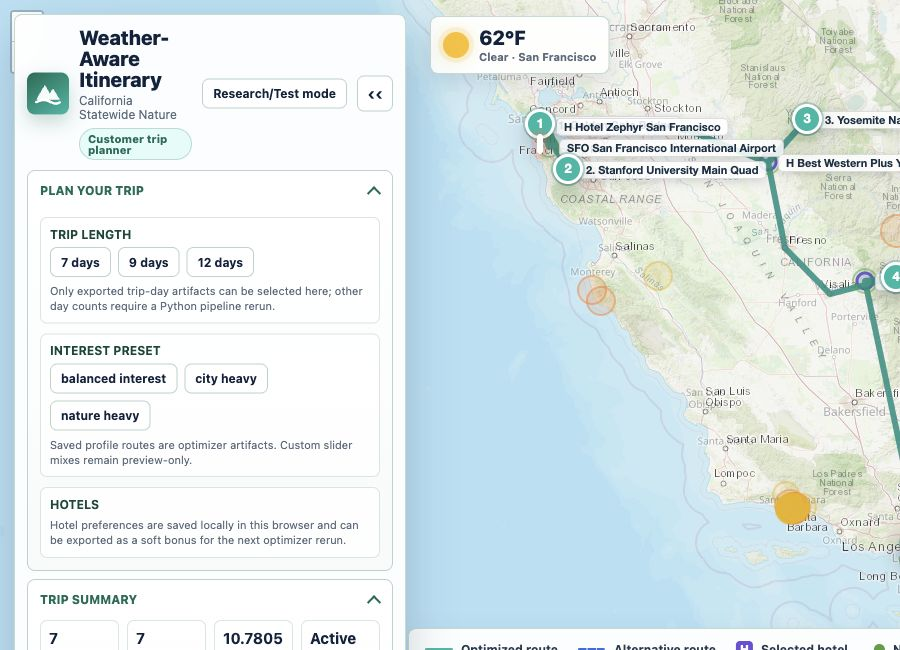
\includegraphics[width=0.92\linewidth]{figures/full_dashboard_screenshot.png}
\caption{Customer-facing dashboard with trip-length controls, interest presets, selected hotel context, weather preview, and map route labels.}
\label{fig:xie-dashboard}
\end{figure}

\begin{figure}[H]
\centering
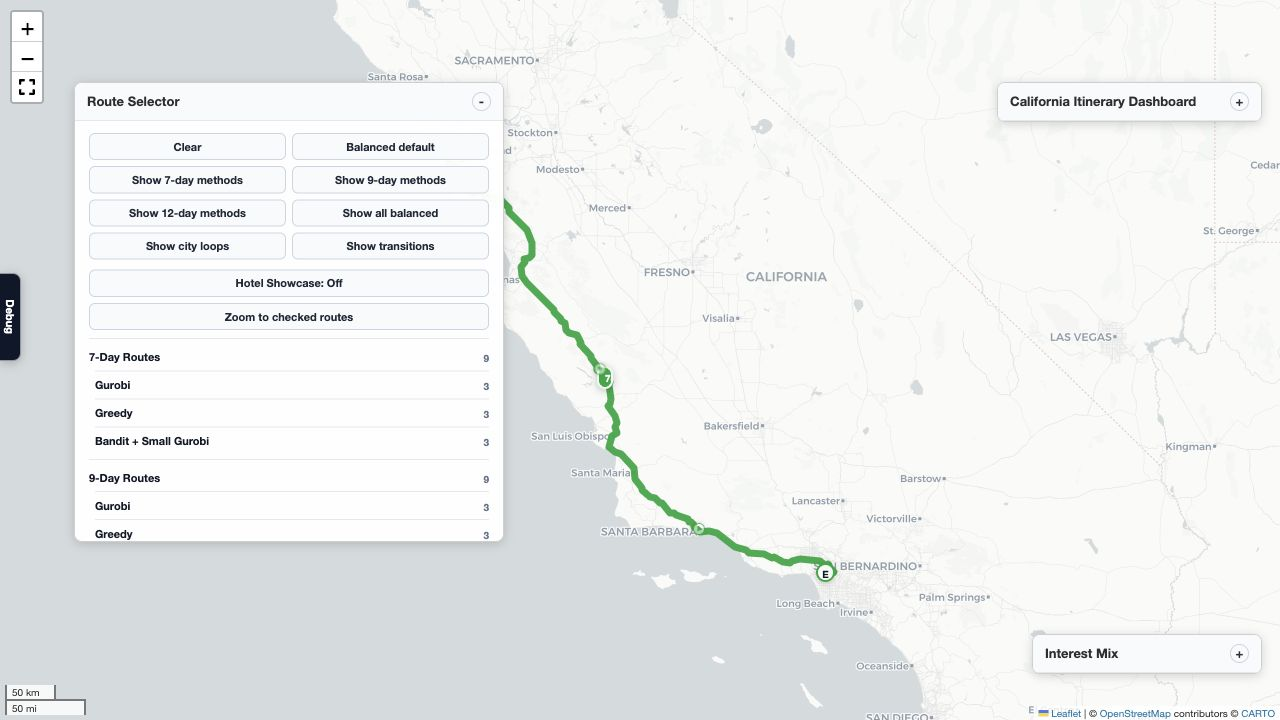
\includegraphics[width=0.92\linewidth]{figures/production_route_map_screenshot.png}
\caption{Production route map showing route-selector controls and comparison-oriented map layers.}
\label{fig:xie-route-map}
\end{figure}

\section*{4. How to Inspect the Current Tool}

\noindent The current repository is:

\begin{center}
\href{https://github.com/Ztang-Yit-Xiaang/weather-aware-travel-itinerary-optimization}{\texttt{github.com/Ztang-Yit-Xiaang/weather-aware-travel-itinerary-optimization}}
\end{center}

\noindent The fastest local inspection path is:

\begin{enumerate}
    \item run \texttt{python scripts/serve\_dashboard.py};
    \item open the printed local URL;
    \item inspect \texttt{index.html}, \texttt{customer.html}, \texttt{research.html}, and \texttt{evaluation.html} under the full dashboard folder;
    \item compare it with \texttt{results/figures/lightweight\_share\_map.html};
    \item review the current output summaries in \texttt{results/outputs/}.
\end{enumerate}

\noindent For a full rerun, the production notebook can be executed with the nature trip config. This separation is intentional: the dashboard is for inspection and communication, while the Python pipeline is responsible for regenerating optimized route artifacts.

\section*{5. Current Pipeline Procedure}

\noindent The current end-to-end procedure is:

\begin{enumerate}
    \item \textbf{Choose scenario and profile.} Select scenario, trip length, budget, pace profile, interest profile, and nature settings from YAML configuration.
    \item \textbf{Build candidate catalog.} Merge or fall back across Yelp-style POIs, OpenStreetMap POIs/hotels, curated social must-go landmarks, NPS or curated nature seeds, and city/nature region metadata.
    \item \textbf{Audit data sources.} Record whether each source came from live APIs, cached data, or curated fallback.
    \item \textbf{Compute utility signals.} Estimate attraction value, interest fit, nature value, scenic value, weather sensitivity, seasonal risk, and detour burden.
    \item \textbf{Construct travel layers.} Prepare within-city and inter-city travel times, hotel-to-attraction times, hotel-to-hotel relocation times, and map geometry.
    \item \textbf{Generate candidate route plans.} Use hierarchical planning and candidate selection to reduce the large search space.
    \item \textbf{Optimize local route segments.} Use Gurobi-style small route repair to produce feasible day-level or city-level routes.
    \item \textbf{Compare methods.} Export comparison files for ranking, greedy, MCDA, TOPSIS, Bayesian/UCB, epsilon-Gurobi, hierarchical Gurobi, and hybrid bandit plus Gurobi repair.
    \item \textbf{Export maps and dashboards.} Generate selected route maps, optional layers, route metrics, POI details, hotel choices, and dashboard assets.
    \item \textbf{Validate artifacts.} Run dashboard and nature-route validation scripts to check consistency between configuration, route data, metadata, and UI assets.
\end{enumerate}

\section*{6. Current Results and Observations}

\noindent The current outputs show that the pipeline can produce feasible route artifacts and method-comparison tables. The current repository and artifacts are available in the \href{https://github.com/Ztang-Yit-Xiaang/weather-aware-travel-itinerary-optimization}{project repository}. The latest generated files show the following snapshot:

\begin{center}
\begin{tabular}{p{0.34\linewidth} p{0.56\linewidth}}
\hline
\textbf{Output file} & \textbf{Current observation} \\
\hline
Method comparison & Compares hierarchical Gurobi, greedy baseline, and hierarchical bandit + small Gurobi repair. The method CSV reports 16 selected attractions for the hybrid repair method and uses about 2041.80 of a 2213.14 buffered budget. \\
Trip-length comparison & Exports 7-day, 9-day, and 12-day route variants over the same Los Angeles to San Francisco corridor. \\
City catalog summary & Contains 228 candidate records across seven California cities, but also shows sparse Yelp coverage outside Santa Barbara. \\
Interest-profile comparison & Compares balanced, nature-heavy, city-heavy, culture-heavy, and history-heavy interest settings. \\
Dashboard route index & Contains 32 route records, including 7 customer-visible options, 25 research-only records, and 27 playable routes. \\
Dashboard validation & The dashboard export validator now passes for the multi-page contract, including customer/research/evaluation pages and richer route metadata. \\
Map validation summary & Reports 97 PASS checks for the production map validation suite. \\
\hline
\end{tabular}
\end{center}

\vspace{0.5em}
\noindent However, these results should be interpreted cautiously. Some methods use different utility scales, some use different candidate scopes, and some reported routes are not directly comparable without further normalization. The system is therefore best understood as a working research prototype rather than a validated final model.

\section*{7. Problems I Would Like Advice On}

\subsection*{7.1 Data Coverage and Data Quality}

\noindent The biggest practical problem is data quality. Recent enrichment audits show that Yelp coverage is sparse outside Santa Barbara, many city-level sources are marked as sparse or fallback, and several live sources are currently offline or disabled. For example, the audit includes statuses such as:

\begin{itemize}
    \item \texttt{yelp\_sparse};
    \item \texttt{overpass\_offline\_missing};
    \item \texttt{wikidata\_offline\_missing} and \texttt{wikipedia\_offline\_missing};
    \item \texttt{open\_meteo\_offline\_missing};
    \item \texttt{nps\_disabled\_curated\_fallback}.
\end{itemize}

\vspace{0.5em}
\noindent This raises a research question: what level of data quality is sufficient for an HCI prototype study? Should the study use a carefully curated dataset for one region, or should it demonstrate robustness across many regions with noisier data?

\vspace{0.5em}
\noindent I also need advice on how to make the data layer more flexible. The future system should be able to switch among live APIs, cached files, curated fallback seeds, regional open-data portals, and possibly agent-discovered datasets without breaking the optimizer. I am not yet sure whether the best design is a strict canonical schema, a plug-in data adapter layer, or a more flexible data contract with explicit confidence and provenance fields.

\subsection*{7.2 Weather and Waiting-Time Validation}

\noindent The current waiting-time model uses review density as a proxy for attraction demand and congestion. This is practical under open-data constraints, but it is not ground-truth queue data. The conversion from reviews to visitor volume also depends on assumptions. I need advice on whether this should be framed as a proof-of-concept contextual signal, or whether I should seek stronger validation data before publication.

\subsection*{7.3 Objective Calibration}

\noindent The objective combines many terms: attraction value, waiting time, travel time, cost, hotel quality, relocation penalty, diversity, nature value, scenic value, weather risk, seasonality risk, and detour penalty. Many weights are currently hand-designed. This is understandable for a prototype, but it may be weak for a CHI paper unless the weights are connected to user preferences or sensitivity analysis.

\vspace{0.5em}
\noindent I would like advice on whether to focus on weight learning, user-adjustable weights, sensitivity analysis, or explanation of tradeoffs.

\subsection*{7.4 Nature-Heavy and Nationwide Planning Need Stronger Data Contracts}

\noindent The nature-aware extension is conceptually implemented, but it still needs stronger data contracts before I can honestly claim robust nationwide behavior. The current California-focused artifacts are useful, but expanding to national parks, multi-state road trips, and city-plus-nature vacations will require the candidate catalog, route graph, optimizer inputs, dashboard outputs, and audit metadata to stay synchronized.

\begin{itemize}
    \item Nature regions need consistent gateway/base-city relationships.
    \item Required anchors need explicit candidate, selected, skipped, or infeasible statuses.
    \item Route artifacts need fresh metadata linking them back to scenario, config, method, and timestamp.
    \item The browser dashboard needs to distinguish saved optimized routes from preview-only routes.
    \item Data-source confidence and fallback status need to travel with each selected stop.
\end{itemize}

\noindent This suggests that the next research/engineering step is not simply adding more places, but defining a flexible data layer that can support many regions without breaking the optimizer's assumptions.

\subsection*{7.5 Dashboard and Artifact Validation}

\noindent The production map validation summary currently reports 97 PASS checks, and the dashboard export validator now passes the newer multi-page dashboard contract. This is encouraging, but I still need to make the validation story clearer. The system has multiple validation layers: map validation, dashboard export validation, nature-route validation, and tests. I would like advice on which validation outputs matter most for a paper and how to report them without overwhelming readers.

\vspace{0.5em}
\noindent This matters because the interface must not mislead users. If a browser preview is approximate while the saved route is optimized by Python, the UI must communicate that distinction clearly and every screenshot/report figure should identify whether it shows a saved route or a preview.

\subsection*{7.6 Scalability of Exact Optimization}

\noindent A nationwide system cannot solve every possible attraction, hotel, and inter-city decision in one exact MIP. The current hybrid strategy is to use candidate selection and hierarchical decomposition, then call small Gurobi repairs. I need advice on how to present this method rigorously: as an engineering heuristic, an approximation framework, or an interactive planning architecture.

\subsection*{7.7 Evaluation Design and Venue Fit}

\noindent The technical system is strong enough to support a study, but the publishable contribution still needs to be narrowed. Possible study directions include:

\begin{itemize}
    \item user trust in optimization-based recommendations;
    \item perceived agency when users can adjust interest bars and constraints;
    \item usefulness of why-selected and why-not-selected explanations;
    \item comparison between optimized routes and ranked-list planning;
    \item whether users understand uncertainty from weather, congestion, and data-source quality.
\end{itemize}

\noindent I would appreciate advice on which of these directions is most realistic and valuable, and which venue family would best match the resulting paper.

\section*{8. Specific Questions for Prof. Xie}

\begin{enumerate}
    \item What should be the main research contribution: the optimization model, the human-centered interface, the explanation design, or the agent-assisted data pipeline?
    \item For a publishable paper, should I prioritize a polished single-region user study or a broader nationwide prototype with less complete data?
    \item How should I handle data-source uncertainty and fallback data in a way that is academically honest but still useful?
    \item How can I make the data pipeline flexible enough to support different cities, states, and nationwide scenarios while still keeping the optimizer inputs clean and reliable?
    \item Is review-density-based waiting-time estimation acceptable as a proxy, or should I simplify the weather component and focus on user interaction?
    \item What evaluation metrics would you recommend for trust, agency, workload, perceived route quality, and explanation usefulness?
    \item Should the browser preview be treated as an interactive explanation tool, while saved routes remain optimization outputs?
    \item How can I best position the future agent component without making the project look like an unconstrained generative-AI itinerary planner?
    \item Which paper submission venues would you recommend for this project? For example, should I consider CHI, IUI, RecSys, UMAP, SIGSPATIAL, HCOMP, or an operations-research decision-support venue?
\end{enumerate}

\section*{9. Proposed Next Steps}

\noindent My proposed next steps are:

\begin{enumerate}
    \item Maintain artifact synchronization: metadata freshness, route-anchor audit rows, dashboard validation, and selected-route/default-route consistency.
    \item Decide whether the publication prototype should focus on California coast, California statewide nature, or another clearer scenario.
    \item Simplify the interface around a small number of interpretable tradeoffs: pace, budget, nature/city/culture/history interest, weather sensitivity, and travel tolerance.
    \item Add explanation fields for why a stop was selected and why high-value alternatives were skipped.
    \item Design a pilot user study comparing optimized interactive planning with a ranked-list or static-map baseline.
    \item Prepare a concise paper outline with clear contribution claims, limitations, and a venue-specific submission plan.
\end{enumerate}

\section*{10. Summary}

\noindent The project has progressed from a course-report optimization notebook into a larger research prototype with configurable scenarios, nature-aware utility, hybrid optimization, route validation, and interactive map/dashboard artifacts. The main challenge now is not only adding more features, but making the system coherent, explainable, validated, and research-ready. I would be grateful for Prof. Xie's suggestions on how to narrow the scope, strengthen the project, and choose an appropriate submission venue.

\end{document}
